% Created 2021-01-24 Sun 22:49
% Intended LaTeX compiler: pdflatex
\documentclass[11pt]{article}
\usepackage[utf8]{inputenc}
\usepackage[T1]{fontenc}
\usepackage{graphicx}
\usepackage{grffile}
\usepackage{longtable}
\usepackage{wrapfig}
\usepackage{rotating}
\usepackage[normalem]{ulem}
\usepackage{amsmath}
\usepackage{textcomp}
\usepackage{amssymb}
\usepackage{capt-of}
\usepackage{hyperref}
\usepackage{minted}
\hypersetup{colorlinks=true, linkcolor=black, filecolor=red, urlcolor=blue}
\usepackage[turkish]{babel}
\author{Eren Hatırnaz}
\date{3 Mayıs 2020}
\title{Yazılım Gündemi - 2020/17\\\medskip
\large 27 Nisan - 3 Mayıs 2020}
\hypersetup{
 pdfauthor={Eren Hatırnaz},
 pdftitle={Yazılım Gündemi - 2020/17},
 pdfkeywords={},
 pdfsubject={},
 pdfcreator={Emacs 27.1 (Org mode 9.3)},
 pdflang={Turkish}}
\begin{document}

\maketitle
\tableofcontents \clearpage\shorthandoff{=}

\begin{center}
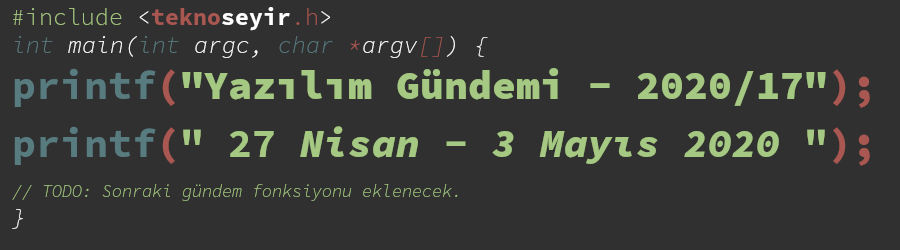
\includegraphics[width=.9\linewidth]{gorseller/yazilim-gundemi-banner.png}
\end{center}

\begin{center}
\href{../16/yazilim-gundemi-2020-16.pdf}{< Önceki Gündem} | \textbf{27 Nisan - 3 Mayıs 2020} | \href{../18/yazilim-gundemi-2020-18.pdf}{Sonraki Gündem >}

\href{https://teknoseyir.com/blog/yazilim-gundemi-2020-17}{TeknoSeyir'de Oku}
\end{center}

\section{Lise öğrencilerine yönelik uluslararası \href{http://meb.gov.tr/lise-ogrencilerine-yonelik-uluslararasi-yazilim-egitimleri-erisime-acildi/haber/20834/tr}{yazılım eğitimleri erişime açıldı}}
\label{sec:org199fd0b}
\begin{center}
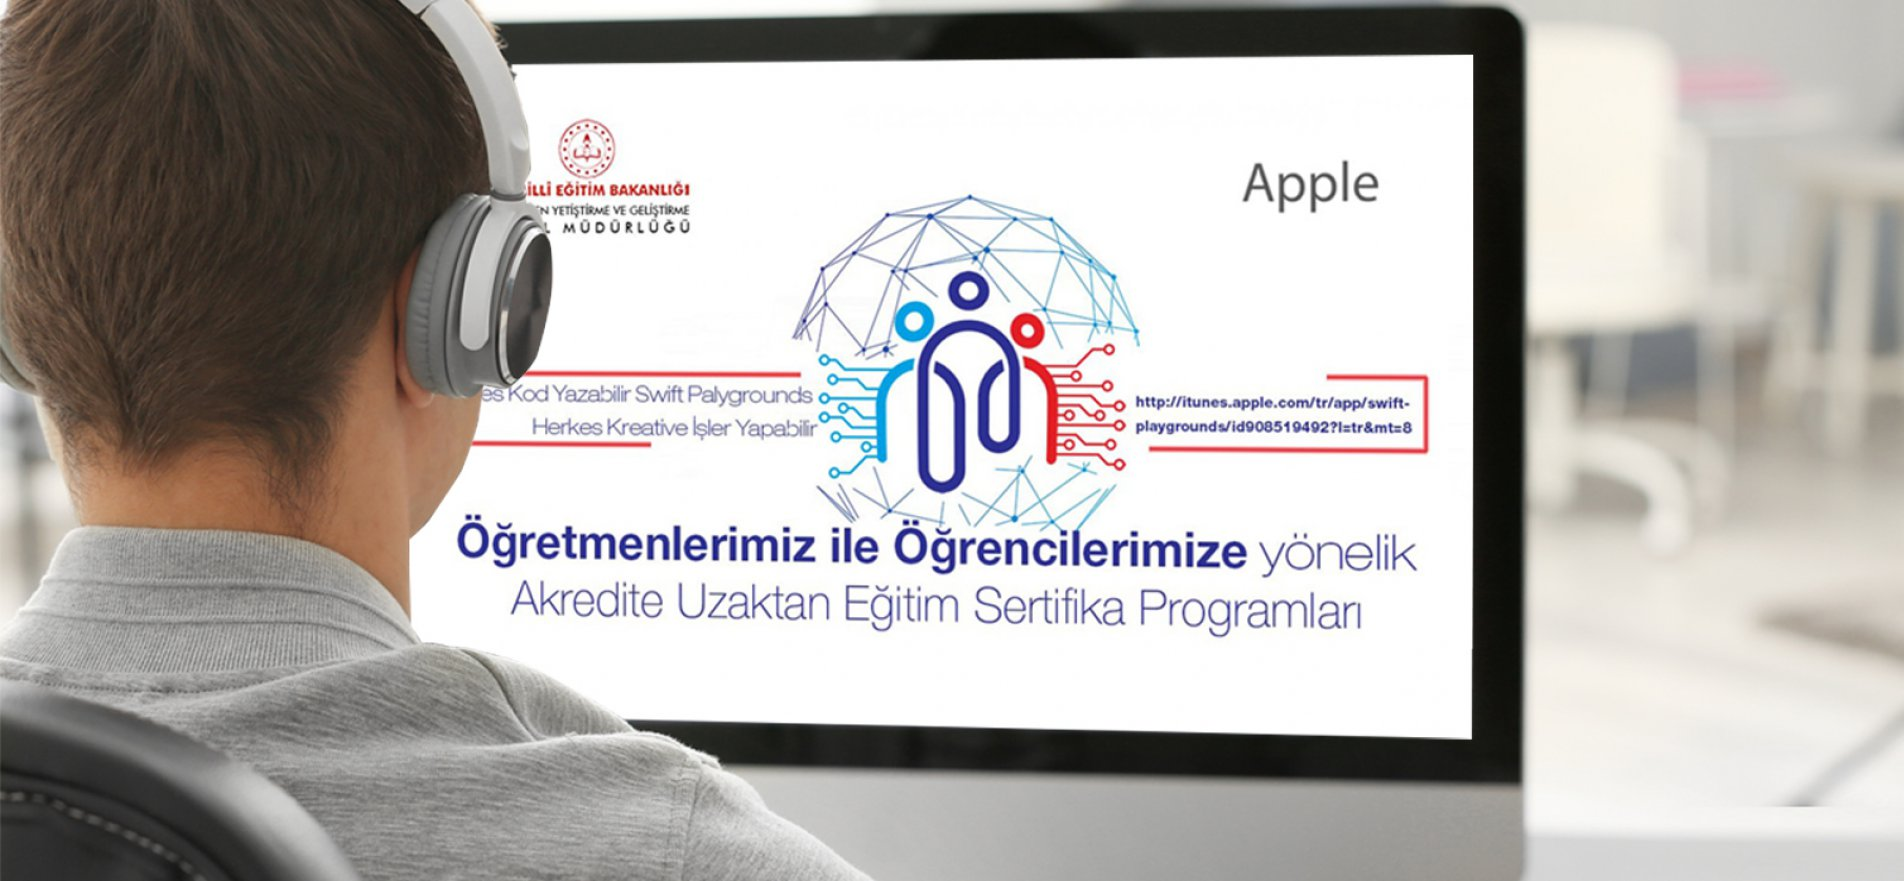
\includegraphics[width=.9\linewidth]{gorseller/meb-yazilim-egitim.png}
\end{center}

Milli Eğitim Bakanlığının web sitesinde bugün yayınlanan duyuruya göre zaten
öğretmenler için devam etmekte olan bazı yazılım geliştirme eğitimleri, lise
öğrencileri için de erişime açılmış.

\begin{quote}
"Öğrencilerimiz için başlatılan bu eğitimlere, Android mobil uygulama
geliştirmek için gerekli teorik bilgiler ile programlama dillerini
öğrenecekleri ve bol bol pratik yaparak eğlenceli ve öğretici uygulamalar
yazacakları üç yeni eğitim daha eklendi." bilgisini veren Selçuk, şunları
kaydetti: "Google iş birliğinde 'Flutter ile Yazılım Geliştirme' ve 'Kotlin
ile Yazılım Geliştirme' android uygulama eğitimleri, Öğretmen Yetiştirme ve
Geliştirme Genel Müdürlüğü Youtube kanalı üzerinden tüm öğrenci ve
öğretmenlerin erişimine açıldı. Google ve Cisco iş birliğinde hazırlanan bu
programlarla öğrencilerin mobil uygulama oluşturma, yapay zeka, gömülü
sistemler, robotik, big data konusundaki bilgi ve becerilerinin artırılmasını
hedefliyoruz."
\end{quote}

Öğretmen Yetiştirme ve Geliştirme Genel Müdürlüğünün YouTube Kanalındaki
yazılım geliştirme videolarını içeren oynatma listelerine aşağıdaki
bağlantılardan ulaşabilirsiniz:
\begin{itemize}
\item \href{https://www.youtube.com/playlist?list=PLVR0OGiP4Ky\_x69HfEbrhlpbGUvpQ3\_JE}{Android Uygulamaları - Kotlin}
\item \href{https://www.youtube.com/playlist?list=PLVR0OGiP4Ky9VQUSthzimF-BqeBp1YWcU}{Android Uygulamaları - Flutter}
\item \href{https://www.youtube.com/playlist?list=PLVR0OGiP4Ky9RKQvi\_ILDN-lmmWxldoa0}{Siber Güvenlik}
\end{itemize}

Ayrıca Cisco tarafından sertifikalı öğretmenler de Python programlama dili
için eğitimler verecekmiş fakat ilgili YouTube kanalında o eğitimleri
bulamadım. Sanırım henüz yayınlanmamış.

"Delphi eğitimi" olayın sonra (bkz: \href{../04/yazilim-gundemi-2020-04.pdf}{Yazılım Gündemi - 2020/04}) bence güzel bir
gelişme bu. Elbette sadece internet üzerinden videolarla olacak iş değil,
farklı eğitimsel içeriklerle ve pratiklerle de desteklenmeli ama başlangıç
için güzel bir adım. Video sayıları henüz az gözüküyor ama anladığım kadarıyla
hepsini birden paylaşmamışlar, her güne ayrı video şeklinde yayınlıyorlar.
İlgili arkadaşlar yukarıdaki bağlantıları takip edebilirler ya da çevresindeki
lise öğrencilerine tavsiye edebilirler.
\section{Visual Studio Online hayatına artık Visual Studio Codespaces \href{https://devblogs.microsoft.com/visualstudio/introducing-visual-studio-codespaces/\#lower-price}{olarak devam edecek}}
\label{sec:org46e4511}
Geçtiğimiz senenin yazılım gündemi yazılarının birinde (bkz: \href{../../2019/yazilim-gundemi-17.pdf}{Yazılım Gündemi -
17}) Microsoft'un "Cloud Geliştirme" çözümü olan Visual Studio Online'ın
tanıtıldığından bahsetmiştim. "Cloud Geliştirme" ortamları giderek daha da
popülerleşirken Microsoft'da bu hizmetinin ismini değiştirdi ve fiyatlarını da
aşağıya çekti.

Kasım ayından bu yana Microsoft aldığı geri bildirimlerle birlikte çoğu
kişinin yüksek özellikli geliştirme ortamlarına ihtiyaç duymadığını
öğrenmişler ve hizmetlerine yeni bir paket eklemişler: Basic. Bu paketde 2
sanal çekirdek, 4GB RAM ve 64GB SSD bulunuyor. Benim de üzerinde çalıştığım
çoğu proje için yeterli bir paket fakat "cloud development" bana pek cazip
gelmiyor. Güncellenen fiyat listesi işe şu şekilde:

\begin{longtable}{|p{5cm}|p{3cm}|p{3cm}|}
\caption{(*): Fiyat/Saat}
\\
\hline
Linux instance tipi & Şimdiki fiyatı(*) & Yeni Fiyat(*)\\
\hline
\endfirsthead
\multicolumn{3}{l}{Önceki sayfadan devam ediyor} \\
\hline

Linux instance tipi & Şimdiki fiyatı(*) & Yeni Fiyat(*) \\

\hline
\endhead
\hline\multicolumn{3}{r}{Devamı sonraki sayfada} \\
\endfoot
\endlastfoot
\hline
Basic (2 çekirdek, 4GB RAM & \$0.24 & \$0.08\\
Standard (4 çekirdek, 8GB RAM) & \$0.45 & \$0.17\\
Premium (8 çekirdek, 16GB RAM) & \$0.87 & \$0.34\\
\hline
\end{longtable}
Fakat yeni fiyatlar hemen yürülüğe girmiyor. Microsoft'un 19 Mayıs'da
düzenleyeceği sanal Build 2020 etkinliğinden sonra yeni fiyatlarla
kullanılmaya devam edilebilecek.

Sıkça soruyorum ama konusu açılmışken yine sorayım: Geliştirme ortamınızı
"cloud development" olarak güncellemeyi düşünüyor musunuz? "Cloud Development"
olayına bakışınız nasıl? Yorumlar bölümünde konuşalım.
\section{Microsoft, Rust/WinRT ön izleme \href{https://blogs.windows.com/windowsdeveloper/2020/04/30/rust-winrt-public-preview/}{sürümünü tanıttı}}
\label{sec:orgacfa055}
Geçtiğimiz yazılım gündemi yazılarında detaylıca değindiğim konular arasında
olmasa da Microsoft'un Rust programlama diline olan ilgiliyle alakalı
haberleri "Diğer Haberler" bölümü altında paylaşmıştım. \href{https://www.rust-lang.org/tr/}{Rust}, Mozilla
tarafından geliştirilen güvenlik ve performans odaklı bir programla dili ve
popülaritesi de gün geçtikçe artmaya devam ediyor. Bu hafta ise Microsoft,
Windows için Rust ile uygulama geliştirmeye yarayan WinRT kütüphanesinin ön
izleme sürümünü \href{https://github.com/microsoft/winrt-rs}{GitHub üzerinde açık kaynak olarak paylaştı}.

Şu anda güncel olarak C++/WinRT üzerinde desteklenen tüm API'ler Rust/WinRT
üzerinde de destekleniyor ve kullanılabiliyor. Yani artık Rust ile Windows
üzerinde masaüstü uygulamalardan, cihaz sürücülerine (driver) kadar birçok
tipte yazılımı geliştirebileceğiz. Microsoft'da örnek olması açısından Rust
ile bir mayın tarlası uygulaması geliştirmiş ve \href{https://github.com/robmikh/minesweeper-rs}{GitHub üzerinde kodlarını
paylaşmış}.

Henüz gerçek uygulamalarda kullanmak için çok erken bir ön izleme sürümü fakat
yeni denizlere açılmayı seven geliştirici arkadaşların ilgisine sunmuş olayım.
Konu hakkında daha detaylı bilgi ve örnekler için konu başlığına eklediğim
bağlantıya tıklayabilirsiniz.

Ayrıca Microsoft'un Rust'a olan ilgisi de devam edecek gibi gözüküyor. Çünkü
Azure takımı da Rust dilini WebAssembly ile birlikte \href{https://www.zdnet.com/article/microsoft-why-we-used-programming-language-rust-over-go-for-webassembly-on-kubernetes-app/}{Kubernetes üzerinde test
ediyormuş}. Önümüzdeki süreçlerde Microsoft'un Rust'a olan ilgisinin ne kadar
süreceğini hep birlikte göreceğiz.
\section{Chrome Web Store, Geliştirici Programı Politikalarını \href{https://blog.chromium.org/2020/04/keeping-spam-off-chrome-web-store.html}{güncelledi}}
\label{sec:orgc81395d}
Google tarafından geliştirilen Chrome web tarayıcısının eklenti mağazası olan
Web Store'da eklenti yayınlarken geçerli olan kurallar bu hafta içerisinde
güncellendi.

Google, yollanan her eklentiyi markete eklemeden önce denetimden geçiriyor.
Güvenlik vb. gibi konular düşünüldüğünde bu çok da normal bir süreç aslında
fakat bazı geliştiriciler sürekli birbirinin benzeri uygulamaları göndererek
bu süreç içerisindeki diğer eklentilerin incelenme sürelerini uzatıyorlarmış.
Yani siz bir eklenti yapıp bunu markete ekletmek istediğinizde bunun için
beklemeniz gereken süre uzuyor. Bu durumun önüne geçmek için Google'da
politikalarını değiştirmeye yoluna gidiyor. Politikalardaki güncellemeler şu
şekilde:

\begin{itemize}
\item Birbirinin aynısı deneyimleri ve fonksiyonları olan eklentiler artık
yayınlanmayacak.
\item Yanıltıcı, yanlış biçimlendirilmiş, açıklayıcı olmayan, alakasız, aşırı
veya uyumsuz meta bilgileri olan eklentiler fakat bunlar sadece eklentinin
açıklamasını kapsamıyor aynı zamanda eklentinin ismi, başlığı, ikonu, ekran
görüntüleri ve promosyon görüntüleri de bu kurallara uymak zorunda.
\item Geliştiriciler Chrome Web Store'daki eklentilerin sıralamalarını
değiştirmeye yönelik hareketlerde bulunamazlar. Sahte incelemeler,
eklentiyi otomatik indiren ve puanlayan botlar vb. şeyler.
\item Sadece başka bir web sitesini, uygulamayı ya da temayı aktifleştirmeye
yarayan eklentiler artık kabul edilmeyecek.
\item Kullanıcılara sürekli spam olarak mesajlar, reklamlar, hedefli saldırılar
(phishing), promosyon gönderen eklentiler yayınlanmayacak.
\end{itemize}

Bu yeni politikların uygulanmasına 27 Ağustos 2020 tarihinde başlanacakmış.
Eğer Chrome Web Store'da yayınlanmış bir eklentiniz varsa yeni politikaları
ihlal edip etmediğinizi kontrol edin. Zira 27 Ağustos itibariyle bu kurallara
uymayan tüm eklentiler marketten kaldırılacaklar.

Daha fazla bilgi için konu başlığına eklediğim bağlantıya ya da Chromium
takımının hazırladığı \href{https://developer.chrome.com/webstore/spam-faq}{Sıkça Sorulan Sorular sayfası}nı ziyaret edebilirsiniz.
\section{TypeScript \href{https://devblogs.microsoft.com/typescript/announcing-typescript-3-9-rc/}{3.9 RC sürümü yayınlandı}}
\label{sec:orge1250c7}
Microsoft tarafından geliştirilen, JavaScript'e derlenebilen tipli programlama
dilin olan TypeScript, bu hafta içerisinde 3.9 Release Candidate sürümüne
kavuştu. Açıkcası uzun bir zamandır front-end teknolojileri ile pek
ilgilenmiyorum dolayısıyla bu haberi de "Diğer Haberler" kısmına taşımıştım ki
son anda anlayabildiğim bir yeni özellik fark ettim. Hız iyileştirmeleri
hakkında zaten fazla bilgi verilmiş, gidip kodları okumak gerekiyor. Editör
iyileştirmelerini de programlama dilinin yapısıyla ilgili olmadığı için
almadım. Öyleyse anladığım özelliği aktarayım size :).

\subsection{\texttt{// @ts-expect-error} yorum satırı \href{https://github.com/microsoft/TypeScript/pull/36014}{Pull Request Sayfası}}
\label{sec:org8729864}
TypeScript kullanarak bir kütüphane yazıyor olduğunu düşünün ve şöyle bir
fonksiyonunuz var:

\begin{minted}[breaklines=true,breakanywhere=true,frame=lines, linenos, label=TypeScript]{typescript}
function hadiBirSeylerOlsun(abc: string, xyz: string) {
    assert(typeof abc === "string");
    assert(typeof xyz === "string");

    // bir şeyler oluyor
}
\end{minted}
Bu fonksiyon iki tane \texttt{string} türünden değer kabul ediyor, biz TypeScript
ile bu fonksiyonu kullanırken \texttt{string} dışında bir türden değişken
gönderirsek TypeScript hata vererek derlenmeyecek, benzer şekilde bu
fonksiyonu JavaScript tarafında kullanmaya çalışırsak da çeşitli hatalar
görüyoruz. Bu durum için test yazmaya çalıştığımızda ise şöyle bir kod
yazabiliriz:
\begin{minted}[breaklines=true,breakanywhere=true,frame=lines, linenos, label=JavaScript]{javascript}
expect(() => {
  hadiBirSeylerOlsun(123, 456);
}).toThrow();
\end{minted}
Fakat bu kod TypeScript'de derlenmeyecektir çünkü fonksiyona \texttt{string} dışında
bir değer gönderdik. İşte bu durumun önlemek için fonksiyonumuzun hemen üst
satırına \texttt{// @ts-expect-error} yorum satırını ekliyoruz ve artık TypeScript
derleyicisi bu fonksiyonun çalıştırılmasıyla bir hata beklendiğini anlayacak
ve bu satırın tip kontrolünü atlayacak.

Bu iş için daha önceden \texttt{ts-ignore} ifadesi kullanılıyormuş sanırım fakat
bazı durumlarda soruna yol açabildiği için bu özel durum için özel bir yorum
satırı işaretleyicisi oluşturmuşlar.

TypeScript 3.9 Release Candidate sürümü ile birlikte gelen diğer özellikler ve
değişiklikler için konu başlığına eklediğim bağlantıya tıklayabilirsiniz.
\section{SourceHut project hub \href{https://sourcehut.org/blog/2020-04-30-the-sourcehut-hub-is-live/}{duyuruldu}}
\label{sec:orgc27168d}
\href{https://sourcehut.org}{SourceHut}, tıpkı diğer uzak git sunucuları (GitHub, GitLab vb.) gibi size git
depolarınızı uzak bir sunucuda tutma imkanı veren bir web sitesi. Tabii ki
artık modern yazılım geliştirme süreçlerinin birer parçası olan CI (Continuous
Integration), proje yönetimi (issue takibi vb.), wiki, kod inceleme (code
review) gibi farklı sorunlara da çözüm üreten servisleri mevcut. Yalnız
SourceHut'ın diğerlerinden farklı bir yani var: sitede JavaScript
kullanılmıyor, her şey sunucu tarafında çalışıyor. Ayrıca \%100 açık kaynak ve
özgür yazılım olarak bir kişi tarafından geliştiriliyor. İlk yazılım gündemi
yazısında bu siteye gelen bir özellikten bahsetmiştim ve benim de çok
beğendiğim bir servis olduğu için ne zamandır tekrar gündemde değinmek için
bahane arıyordum :).

SourceHut bu hafta içerisinde "project hub" ismini verdiği yeni servisini
duyurdu. Bu yeni servisin ne işe yaradığını anlamak için öncesince
SourceHut'ın arkasındaki UNIX felsefesini bilmek gerek. GNU/Linux
kullananların da aşina olduğu üzere işletim sistemiyle birlikte gelen
araçların çoğu "sadece bir şeyi yap ama en iyi yap" anlayışıyla geliştirilmiş
araçlardır. Dolayısıyla elinizin altında birbiriyle kombinleyebileceğiniz bir
sürü araç olmuş oluyor. Örneğin \texttt{cat} komutu sadece bir dosyanın içeriğini
yazdırmaya yararken, \texttt{grep} komutu bir dosya içerisinde metin arama gibi
işlemleri yapabiliyor. İşte SourceHut da bu yaklaşımla geliştiriliyor. Sadece
bir işi en iyi şekilde yapmaya çalışan birçok alt servis var. Git depolarınızı
barındırmak için \href{https://git.sr.ht}{git.sr.ht}, issue takibi vb. işler için \href{https://todo.sr.ht}{todo.sr.ht}, CI
işlemleri için \href{https://builds.sr.ht}{builds.sr.ht} vb. birçok alt servis bulunmakta. Hepsini görmek
için \href{https://sourcehut.org}{sourcehut.org} adresini ziyaret edebilirsiniz.

Yani oluşturduğunuz bir git deposu sadece git deposu olma işini yapıyor. Issue
takip vb. diğer işler için diğer alt servislerden oluşturmanız gerekiyor. İşte
"project hub" ise bütün bu alt servisleri GitHub ve GitLab'dan alıştığımız
gibi tek bir sayfada birleştiriyor. Fakat yanlış anlaşılmasın bu alt servisler
birleşip tek hale gelmiyor, sadece bir projeye ait tüm alt kaynaklar bir
sayfada toplanıyor, isterseniz tıklayarak o alt servisteki işlemlerinize
gidebiliyorsunuz. Üstelik bir projeye istediğiniz kadar alt servis
ekleyebiliyorsunuz, mesela bir uygulamanın Android ve iOS sürümlerini ayrı
ayrı git depolarında tutuyorsanız onları da tek bir projeye
ekleyebiliyorsunuz.

\begin{figure}[htbp]
\centering
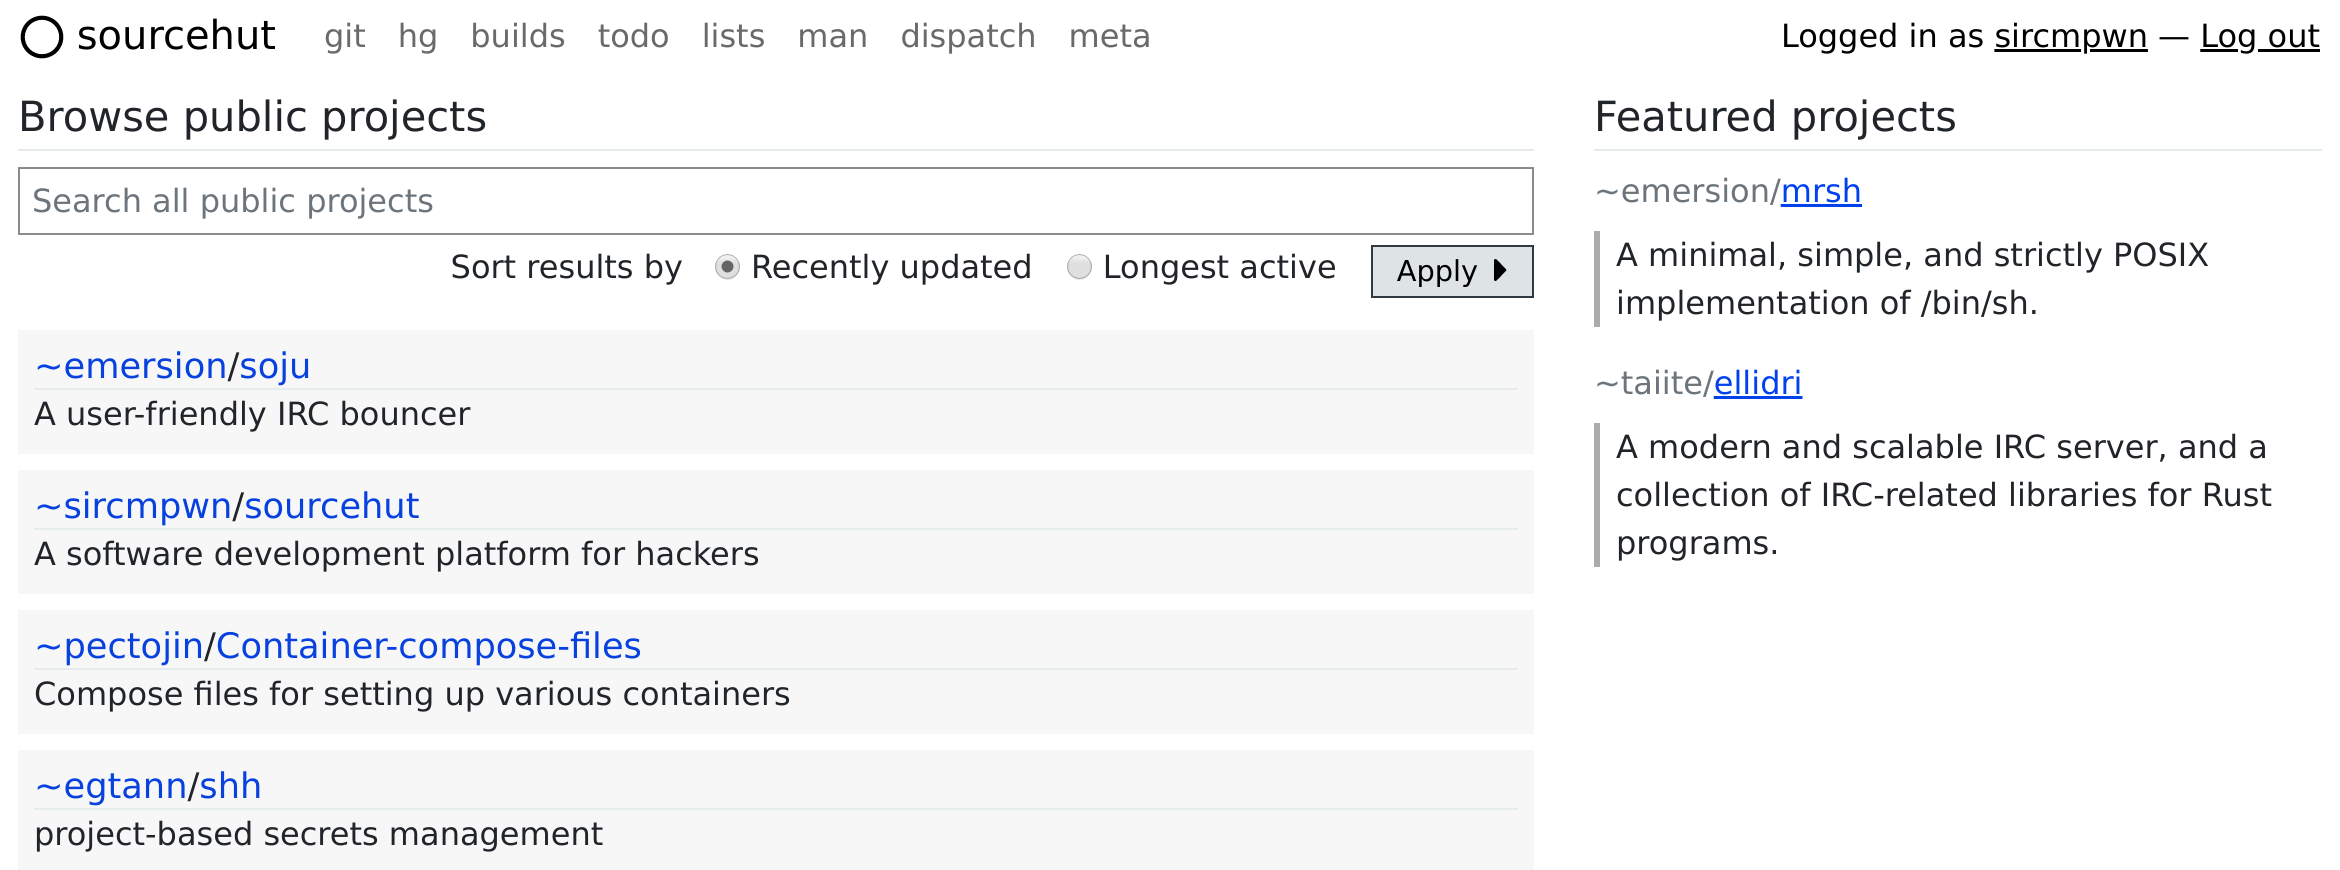
\includegraphics[width=.9\linewidth]{gorseller/sourcehut-project-hub.png}
\caption{Örnek için SourceHut'ın tüm alt servisleriyle birlikte kodlarını barındıran \href{https://sr.ht/\~sircmpwn/sourcehut/}{bu proje sayfasını ziyaret edebilirsiniz}.}
\end{figure}

SourceHut dışından gelenler için böyle bir sayfanın olması çok önemliydi ve
sonunda eklediler. Siz de benim gibi UNIX felsefesinden hoşlanan ve GNU/Linux
araçları gibi basit ve sade araçları kullanmayı seviyorsanız mutlaka
\href{https://sourcehut.org}{SourceHut}'a bir göz atın. Ayrıca tek kişi tarafından geliştirildiğini aklınıza
getirerek bağış yapmayı da düşünebilirsiniz.
\section{Yaklaşan Online Etkinlikler \#EvdeKal}
\label{sec:org47e30e1}
\begin{longtable}{|p{9.5cm}|l|}
\hline
Etkinlik İsmi & Tarihi\\
\hline
\endfirsthead
\multicolumn{2}{l}{Önceki sayfadan devam ediyor} \\
\hline

Etkinlik İsmi & Tarihi \\

\hline
\endhead
\hline\multicolumn{2}{r}{Devamı sonraki sayfada} \\
\endfoot
\endlastfoot
\hline
\href{https://kommunity.com/tracikkaynak/events/acik-seminer-14-gun-nlp-101-dogal-dil-islemeye-giris-7194f676}{Açık Seminer 14. Gün: NLP 101: Doğal Dil İşlemeye Giriş} & 5 Mayıs 14:00\\
\href{https://kommunity.com/akademi/events/network-uzerinden-tehdit-avciligi-komuta-kontrol-baglantisinin-tespiti-f6ca2346}{Network Üzerinden Tehdit Avcılığı - Komuta Kontrol} & 5 Mayıs 16:30\\
\href{https://kommunity.com/tracikkaynak/events/acik-seminer-15-gun-bankacilik-finans-alaninda-dogal-dil-isleme-d9e0d4a5}{Açık Seminer 15. Gün: Bankacılık \& Finans Alanında Doğal Dil İşleme} & 6 Mayıs 14:00\\
\href{https://kommunity.com/cloud-and-serverless-turkey/events/ramazan-ozel-4-aws-bulut-altyapisi-bilesenleri-8fe02b6e}{AWS Bulut Altyapısı Bileşenleri} & 6 Mayıs 23:00\\
\href{https://kommunity.com/cozumpark/events/siber-koruma-cozumleri-webinari-4effd358}{Siber Koruma Çözümleri Webinarı} & 7 Mayıs 14:00\\
\href{https://kommunity.com/tracikkaynak/events/acik-seminer-16-gun-bilissel-hizmetler-ile-turkce-chatbot-olusturma-df205099}{Açık Seminer 16. Gün: Bilişsel Hizmetler ile Türkçe Chatbot} & 7 Mayıs 14:00\\
\href{https://kommunity.com/devops-turkiye/events/high-available-kubernetes-clusters-with-kops-e2728634}{High Available Kubernetes clusters with KOPS} & 7 Mayıs 22:00\\
\href{https://kommunity.com/tracikkaynak/events/acik-seminer-17-gun-dogal-dil-isleme-urunleri-ve-kullanim-alanlari-c9c008c2}{Açık Seminer 17. Gün: Doğal Dil İşleme Ürünleri ve Kullanım Alanları} & 8 Mayıs 14:00\\
\href{https://kommunity.com/dotnet-istanbul/events/net-core-grpc-servislerini-tarayici-uygulamalarindan-tuketmek-16e940d0}{.NET Core gRPC Servislerini Tarayıcı Uygulamalarından Tüketmek} & 8 Mayıs 22:00\\
\href{https://kommunity.com/devnot-yazilimci-bulusmalari/events/react-native-vs-flutter-02a9d600}{React Native vs. Flutter} & 9 Mayıs 22:00\\
\href{https://kommunity.com/cloud-and-serverless-turkey/events/ramazan-ozel-5-bulutta-ve-kendi-sunucularinizda-kubernetes-dfec6279}{Bulutta ve kendi sunucularınızda Kubernetes} & 9 Mayıs 23:00\\
\href{https://kommunity.com/cloud-and-serverless-turkey/events/kubernetes-hands-on-2-what-is-deployment-pod-and-service-06b07bda}{Kubernetes Hands-On no.2: What is deployment, pod and service?} & 10 Mayıs 13:30\\
\hline
\end{longtable}
\section{Diğer Haberler}
\label{sec:org7246ad6}
\begin{itemize}
\item \href{https://www.jetbrains.com/academy/}{JetBrains Academy}, COVID-19 pandemisi boyunca \href{https://techcrunch.com/2020/05/01/jetbrains-academy-for-learning-code-launches-for-free-during-covid-19-pandemic/}{ücretsiz oldu}.
\item Facebook Yapay Zeka takımı chat botlarıyla ilgili \href{https://ai.facebook.com/blog/state-of-the-art-open-source-chatbot}{detaylı blog yazısı
yayınladı}.
\item Microsoft, yeni bir meta programlama \href{https://devblogs.microsoft.com/dotnet/introducing-c-source-generators/}{aracı tanıttı: C\# Source Generators}.
\item DigitalOcean özel ağlar için \href{https://blog.digitalocean.com/vpc-trust-platform/}{yeni hizmetini duyurdu}: \href{https://www.digitalocean.com/products/vpc}{Virtual Private Cloud}.
\item Google Cloud, yeni metadata yönetim \href{https://cloud.google.com/blog/products/data-analytics/data-catalog-metadata-management-now-generally-available}{servisini genel erişilebilir yaptı}: \href{https://cloud.google.com/data-catalog}{Data
Catalog}
\item Determined AI, derin öğrenme platformunu \href{https://determined.ai/blog/ai-infrastructure-for-everyone/}{açık kaynak hale getirdi}. \href{https://github.com/determined-ai/determined/}{GitHub
Deposu}
\item JetBrains, WebStorm IDE'sinin \href{https://blog.jetbrains.com/webstorm/2020/04/webstorm-2020-1-1}{2020.1.1 sürümünü yayınladı}.
\item Yeni bir API tasarlama aracı \href{https://insomnia.rest/blog/introducing-designer}{açık kaynak olarak duyuruldu}: \href{https://insomnia.rest/products/designer/}{Insomnia
Designer}. \href{https://github.com/Kong/insomnia}{GitHub Deposu}
\item Amazon Web Services yeni veri merkezini açtı: \href{https://aws.amazon.com/about-aws/whats-new/2020/04/announcing-the-new-aws-europe-milan-region/}{Europe (Milan)}.
\item \href{https://www.khronos.org/news/press/khronos-group-releases-opencl-3.0}{OpenCL 3.0 sürümü yayınlandı}.
\item Redis \href{http://antirez.com/news/132}{6.0.0 sürümü yayınlandı}.
\item Açık kaynak proje yönetim sistemi Leantime \href{https://leantime.io/2020/04/29/leantime-v2-1-released-\%25F0\%259F\%259A\%2580\%25F0\%259F\%259A\%2580\%25F0\%259F\%259A\%2580/}{v2.1 sürümünü yayınladı}.
\item VueJS \href{https://github.com/vuejs/vue-next/releases/tag/v3.0.0-beta.7}{v3.0.0 Beta 7 sürümü yayınlandı}.
\item D programlama dilinin \href{https://dlang.org/changelog/2.092.0.html}{2.092.0 Beta sürümü yayınlandı}.
\item AMD Programcı Kılavuzu \href{https://www.phoronix.com/scan.php?page=news\_item\&px=AMD-PRM-PCID-PKEY}{güncellendi}.
\item TypeScript için fonksiyonel programlama kütüphanesi Pruify, \href{https://gigobyte.github.io/purify/changelog/0.15/}{v0.15 sürümünü
yayınladı}. \href{https://github.com/gigobyte/purify}{GitHub Deposu}
\item Microsoft, Shader Conductor \href{https://www.phoronix.com/scan.php?page=news\_item\&px=Microsoft-Shader-Conductor-0.3}{0.3 sürümünü yayınladı}. \href{https://github.com/microsoft/ShaderConductor}{GitHub Deposu}
\item XMake \href{https://tboox.org/2020/04/27/xmake-update-v2.3.3/}{v2.3.3 sürümü yayınlandı}. \href{https://github.com/xmake-io/xmake}{GitHub Deposu}
\item odo \href{https://github.com/openshift/odo/releases/tag/v1.2.0}{v1.2.0 sürümü yayınlandı}.
\item NeutralinoJS \href{https://github.com/neutralinojs/neutralinojs/releases/tag/v1.4.0}{v1.4.0 yayınlandı}.
\end{itemize}
\section{Lisans}
\label{sec:orgefc98d0}
\begin{center}
\begin{center}

\includegraphics[height=1.5cm]{../../../img/CC_BY-NC-SA_4.0.png}
\end{center}

\href{yazilim-gundemi-2020-17.pdf}{Yazılım Gündemi - 2020/17} yazısı \href{https://erenhatirnaz.github.io}{Eren Hatırnaz} tarafından \href{http://creativecommons.org/licenses/by-nc-sa/4.0/}{Creative Commons
Atıf-GayriTicari-AynıLisanslaPaylaş 4.0 Uluslararası Lisansı} (CC BY-NC-SA 4.0)
ile lisanslanmıştır.
\end{center}
\end{document}
